\documentclass[12pt,a4paper]{article}
\usepackage[utf8]{inputenc}
\usepackage[spanish]{babel}
\usepackage{graphicx}
\usepackage{geometry}
\usepackage{hyperref}
\usepackage{listings}
\usepackage{xcolor}
\usepackage{float}
\usepackage{array}
\usepackage{booktabs}
\usepackage{fancyhdr}
\usepackage{setspace}
\usepackage{pdflscape}

\geometry{left=2.5cm, right=2.5cm, top=2.5cm, bottom=2.5cm}
\setlength{\headheight}{14.5pt}
\setstretch{1.5}

\lstset{
    language=Python,
    basicstyle=\footnotesize\ttfamily,
    keywordstyle=\color{blue},
    commentstyle=\color{gray},
    stringstyle=\color{red},
    numbers=left,
    numberstyle=\tiny,
    frame=single,
    breaklines=true,
    tabsize=4
}

\pagestyle{fancy}
\fancyhf{}
\fancyhead[L]{PC4 - Programaci\'on Orientada a Objetos}
\fancyhead[R]{\thepage}
\renewcommand{\headrulewidth}{0.4pt}

\begin{document}

\onecolumn
\begin{titlepage}
    \centering
    \vspace*{2cm}
    {\Huge \textbf{Prototipo Zoom}}\\[0.5cm]
    {\Large Sistema de Videoconferencia por Sockets}\\[1.5cm]
    {\large \textbf{PC4 - SW403U - Programaci\'on Orientada a Objetos}}\\[0.5cm]
    {\large Universidad Nacional de Ingeniería}\\[0.3cm]
    {\large Facultad de Ingenier\'ia Industrial y Sistemas}\\[2cm]

    \begin{tabular}{ll}
        \textbf{Integrantes:} & \\
        & \\ Yampufe Pau Héctor Alonso - 20240310I
        & \\ Romaní Cuyo Gabriel Alberto - 20242045K
        & \\ Tasayco Portello Luis Antonio - 20240307H
    \end{tabular}\\[2cm]

    \textbf{Docente: CISNEROS NAPRAVNIK YAN EDUARDO}\\[1.8cm]

    \today
\end{titlepage}

\tableofcontents
\newpage

\section{Introducci\'on}

El presente documento describe el dise\~no e implementaci\'on de un \textbf{prototipo acad\'emico de videoconferencia} inspirado en Zoom, desarrollado en Python como parte del curso de Programaci\'on Orientada a Objetos (PC4).

El sistema emplea una arquitectura \textbf{cliente-servidor} basada en \textbf{sockets TCP} con un protocolo de mensajes en formato \textbf{JSON}. Cuenta con autenticaci\'on de usuarios, creaci\'on y gesti\'on de salas virtuales, chat en tiempo real, transferencia de archivos y transmisi\'on de video desde la c\'amara web.

\section{Objetivos}

\begin{itemize}
    \item Aplicar los principios de la POO: herencia, encapsulamiento, polimorfismo.
    \item Implementar una arquitectura cliente-servidor mediante sockets TCP.
    \item Desarrollar un protocolo de comunicaci\'on propio basado en JSON.
    \item Integrar m\'ultiples funcionalidades: login, salas, chat, archivos y video.
    \item Utilizar SQLite para la persistencia de informaci\'on.
    \item Emplear concurrencia con \texttt{threading} para atender m\'ultiples clientes.
\end{itemize}

\section{Tecnolog\'ias Utilizadas}

\begin{itemize}
    \item \textbf{Lenguaje:} Python 3.10+
    \item \textbf{Interfaz gr\'afica:} Tkinter
    \item \textbf{Comunicaci\'on:} Sockets TCP (RFC 793)
    \item \textbf{Protocolo de mensajes:} JSON sobre TCP (RFC 8259), delimitado por \verb|\n|
    \item \textbf{Base de datos:} SQLite 3
    \item \textbf{Concurrencia:} \texttt{threading} (modelo de hilos POSIX)
    \item \textbf{Video:} OpenCV 4.x (backend MJPEG) o ffmpeg (V4L2 en Linux)
    \item \textbf{Audio:} PortAudio v19 mediante \texttt{sounddevice} (PCM 16\,bit, 16\,kHz mono)
    \item \textbf{Archivos:} transferencia binaria codificada en Base64 (RFC 4648)
    \item \textbf{Seguridad:} hash SHA-256 para contrase\~nas (FIPS 180-4)
    \item \textbf{Im\'agenes:} Pillow (PIL Fork)
\end{itemize}

\section{Arquitectura del Sistema}

El sistema sigue un modelo cliente-servidor. El servidor centraliza las conexiones y act\'ua como intermediario. Cada cliente se conecta mediante TCP y el servidor asigna un hilo independiente por conexi\'on.

\IfFileExists{imagenes/arquitectura.png}{%
\begin{figure}[htbp]
    \centering
    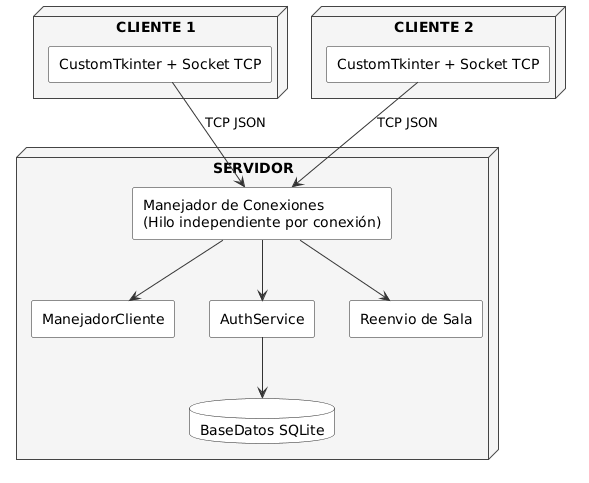
\includegraphics[width=0.9\textwidth]{imagenes/arquitectura.png}
    \caption{Diagrama de arquitectura del sistema}
\end{figure}
}{}

\section{Base de Datos}

La base de datos SQLite contiene las siguientes tablas:

\begin{table}[htbp]
    \centering
    \begin{tabular}{p{3.5cm}p{10cm}}
    \toprule
    \textbf{Tabla} & \textbf{Columnas} \\
    \midrule
    Usuarios          & IdUsuario, Nombres, Correo, PasswordHash, Rol, Activo \\
    Salas             & IdSala, CodigoSala, Nombre, IdHost, Estado, FechaCreacion \\
    ParticipantesSala & IdParticipante, IdSala, IdUsuario, Estado, FechaIngreso \\
    SolicitudesSala   & IdSolicitud, IdSala, IdUsuario, Estado, FechaSolicitud \\
    Mensajes          & IdMensaje, IdSala, IdUsuario, Contenido, FechaEnvio \\
    ArchivosCompartidos & IdArchivo, IdSala, IdUsuario, NombreArchivo, RutaArchivo, Tamano, FechaSubida \\
    \bottomrule
    \end{tabular}
    \caption{Tablas de la base de datos}
\end{table}

\section{Diagrama Entidad-Relaci\'on}

\begin{figure}[H]
    \centering
    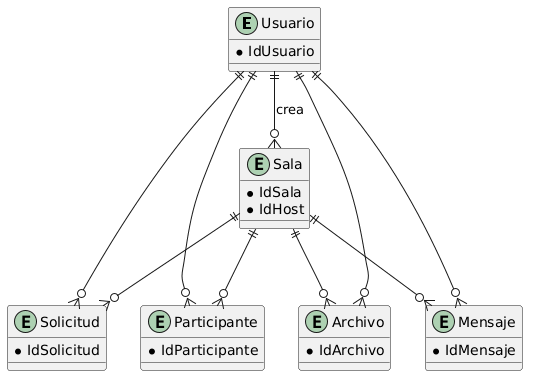
\includegraphics[width=0.95\textwidth]{imagenes/Entidad-Relacion.png}
    \caption{Diagrama Entidad-Relaci\'on de la base de datos}
\end{figure}

\section{Diagrama de Casos de Uso}

\IfFileExists{imagenes/casos_de_uso.png}{%
\begin{figure}[H]
    \centering
    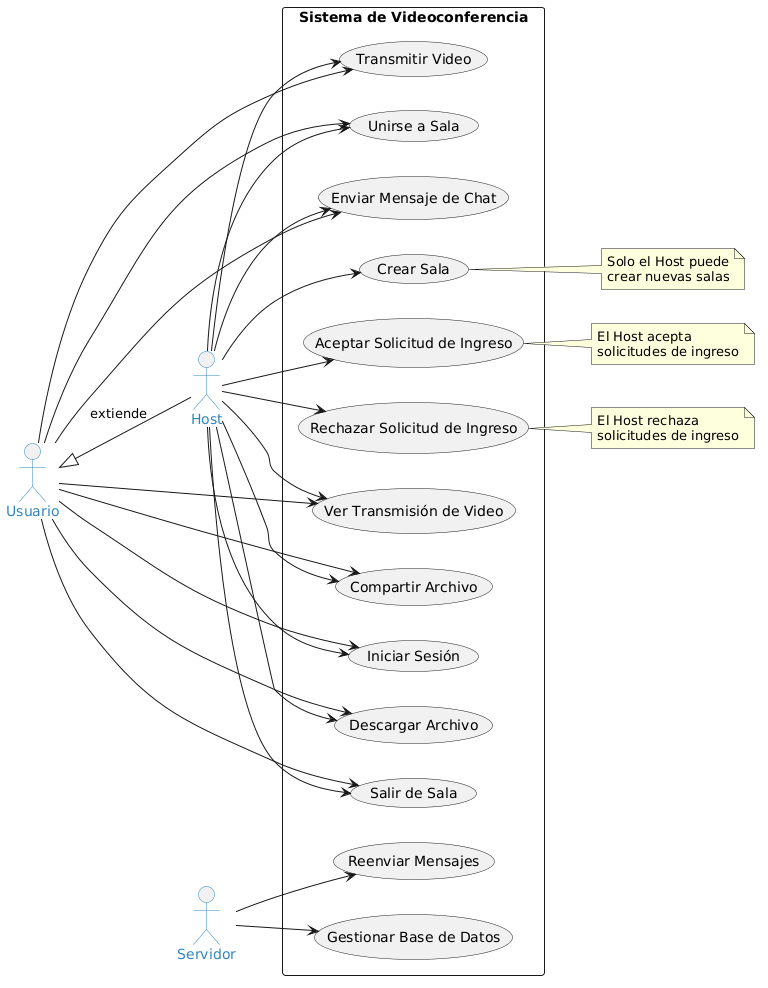
\includegraphics[width=0.9\textwidth]{imagenes/casos_de_uso.png}
    \caption{Diagrama de casos de uso del sistema}
\end{figure}
}{}

\section{Especificaci\'on de Casos de Uso}

Se describen a continuaci\'on los casos de uso principales del sistema.

\subsection*{CU-01: Iniciar Sesi\'on}
\begin{table}[H]
\centering
\small
\begin{tabular}{p{3.5cm}p{10cm}}
\toprule
\textbf{Campo} & \textbf{Descripci\'on} \\
\midrule
\textbf{Actor} & Usuario registrado \\
\textbf{Precondici\'on} & El servidor est\'a activo y el usuario tiene cuenta en el sistema \\
\textbf{Flujo principal} &
  1. El usuario ingresa correo y contrase\~na. \newline
  2. El cliente env\'ia \texttt{LOGIN\_REQUEST} al servidor. \newline
  3. El servidor valida las credenciales con hash SHA-256. \newline
  4. El servidor responde con \texttt{LOGIN\_RESPONSE (status: success)}. \newline
  5. El cliente muestra la pantalla principal. \\
\textbf{Flujo alternativo} & Si las credenciales son incorrectas, el servidor responde con \texttt{status: error} y se muestra un mensaje al usuario. \\
\textbf{Postcondici\'on} & El usuario queda autenticado y puede crear o unirse a salas. \\
\bottomrule
\end{tabular}
\caption{CU-01: Iniciar Sesi\'on}
\end{table}

\subsection*{CU-02: Crear Sala}
\begin{table}[H]
\centering
\small
\begin{tabular}{p{3.5cm}p{10cm}}
\toprule
\textbf{Campo} & \textbf{Descripci\'on} \\
\midrule
\textbf{Actor} & Usuario autenticado (rol Host) \\
\textbf{Precondici\'on} & El usuario ha iniciado sesi\'on exitosamente \\
\textbf{Flujo principal} &
  1. El usuario presiona ``Crear Sala''. \newline
  2. El cliente genera un c\'odigo alfanum\'erico de 6 caracteres. \newline
  3. El cliente env\'ia \texttt{CREATE\_ROOM} con c\'odigo y nombre. \newline
  4. El servidor registra la sala en la BD y asigna al usuario como host. \newline
  5. El cliente accede directamente a la sala como administrador. \\
\textbf{Flujo alternativo} & Si el c\'odigo ya existe, el servidor retorna error y el cliente intenta con otro c\'odigo. \\
\textbf{Postcondici\'on} & La sala queda activa en la base de datos y el host puede gestionar participantes. \\
\bottomrule
\end{tabular}
\caption{CU-02: Crear Sala}
\end{table}

\subsection*{CU-03: Unirse a Sala}
\begin{table}[H]
\centering
\small
\begin{tabular}{p{3.5cm}p{10cm}}
\toprule
\textbf{Campo} & \textbf{Descripci\'on} \\
\midrule
\textbf{Actor} & Usuario autenticado \\
\textbf{Precondici\'on} & Existe una sala activa con el c\'odigo ingresado \\
\textbf{Flujo principal} &
  1. El usuario ingresa el c\'odigo de sala y presiona ``Unirse''. \newline
  2. El cliente env\'ia \texttt{JOIN\_ROOM\_REQUEST}. \newline
  3. El servidor notifica al host con \texttt{WAITING\_ROOM\_UPDATE}. \newline
  4. El host admite al usuario (\texttt{ADMIT\_USER}). \newline
  5. El servidor notifica al invitado y lo agrega a la sala. \\
\textbf{Flujo alternativo} & Si el host rechaza (\texttt{REJECT\_USER}), el cliente recibe notificaci\'on de rechazo y regresa al men\'u. \\
\textbf{Postcondici\'on} & El usuario es participante activo de la sala. \\
\bottomrule
\end{tabular}
\caption{CU-03: Unirse a Sala}
\end{table}

\subsection*{CU-04: Enviar Archivo}
\begin{table}[H]
\centering
\small
\begin{tabular}{p{3.5cm}p{10cm}}
\toprule
\textbf{Campo} & \textbf{Descripci\'on} \\
\midrule
\textbf{Actor} & Participante de la sala \\
\textbf{Precondici\'on} & El usuario est\'a dentro de una sala activa \\
\textbf{Flujo principal} &
  1. El usuario presiona ``Archivo'' y selecciona un fichero. \newline
  2. El cliente codifica el archivo en Base64 y lo fragmenta en chunks de 1500 bytes. \newline
  3. Env\'ia \texttt{FILE\_START}, los \texttt{FILE\_CHUNK} y finalmente \texttt{FILE\_END}. \newline
  4. Los receptores son consultados si desean descargar el archivo. \newline
  5. El receptor acepta y el archivo se reconstruye y guarda en \texttt{descargas/}. \\
\textbf{Flujo alternativo} & Si el receptor rechaza la descarga, el archivo no se guarda en ese cliente. \\
\textbf{Postcondici\'on} & El archivo queda disponible en el equipo de los receptores que aceptaron. \\
\bottomrule
\end{tabular}
\caption{CU-04: Enviar Archivo}
\end{table}

\section{Diccionario de Datos}

Se describe cada atributo relevante de las entidades principales del sistema.

\subsection*{Tabla: Usuarios}
\begin{table}[H]
\centering
\small
\begin{tabular}{p{3cm}p{2cm}p{8.5cm}}
\toprule
\textbf{Campo} & \textbf{Tipo} & \textbf{Descripci\'on} \\
\midrule
IdUsuario & INTEGER & Clave primaria autoincrementable. Identificador \'unico del usuario. \\
Nombres & TEXT & Nombre completo del usuario. No puede ser nulo. \\
Correo & TEXT & Direcci\'on de correo electr\'onico. Debe ser \'unica en el sistema. \\
PasswordHash & TEXT & Hash SHA-256 de la contrase\~na en hexadecimal. Nunca se almacena texto plano. \\
Rol & TEXT & Rol del usuario: \texttt{Host} o \texttt{Usuario}. Valor por defecto: \texttt{Usuario}. \\
Activo & INTEGER & Indicador booleano: 1 = activo, 0 = inactivo (baja l\'ogica). \\
\bottomrule
\end{tabular}
\caption{Diccionario de datos -- Usuarios}
\end{table}

\subsection*{Tabla: Salas}
\begin{table}[H]
\centering
\small
\begin{tabular}{p{3cm}p{2cm}p{8.5cm}}
\toprule
\textbf{Campo} & \textbf{Tipo} & \textbf{Descripci\'on} \\
\midrule
IdSala & INTEGER & Clave primaria autoincrementable. \\
CodigoSala & TEXT & C\'odigo alfanum\'erico de 6 caracteres generado en el cliente. Debe ser \'unico. \\
Nombre & TEXT & Nombre descriptivo de la sala. \\
IdHost & INTEGER & Clave for\'anea a \texttt{Usuarios}. Usuario que cre\'o y administra la sala. \\
Estado & TEXT & Estado de la sala: \texttt{Activa} o \texttt{Cerrada}. Valor por defecto: \texttt{Activa}. \\
FechaCreacion & TEXT & Fecha y hora de creaci\'on en formato ISO 8601 (UTC). \\
\bottomrule
\end{tabular}
\caption{Diccionario de datos -- Salas}
\end{table}

\subsection*{Tabla: SolicitudesSala}
\begin{table}[H]
\centering
\small
\begin{tabular}{p{3cm}p{2cm}p{8.5cm}}
\toprule
\textbf{Campo} & \textbf{Tipo} & \textbf{Descripci\'on} \\
\midrule
IdSolicitud & INTEGER & Clave primaria autoincrementable. \\
IdSala & INTEGER & Clave for\'anea a \texttt{Salas}. Sala a la que se solicita ingreso. \\
IdUsuario & INTEGER & Clave for\'anea a \texttt{Usuarios}. Usuario que solicita ingresar. \\
Estado & TEXT & Estado de la solicitud: \texttt{Pendiente}, \texttt{Admitido} o \texttt{Rechazado}. \\
FechaSolicitud & TEXT & Fecha y hora de la solicitud en formato ISO 8601. \\
\bottomrule
\end{tabular}
\caption{Diccionario de datos -- SolicitudesSala}
\end{table}

\section{Diagrama de Secuencia}

\IfFileExists{imagenes/secuencia.png}{%
\begin{figure}[H]
    \centering
    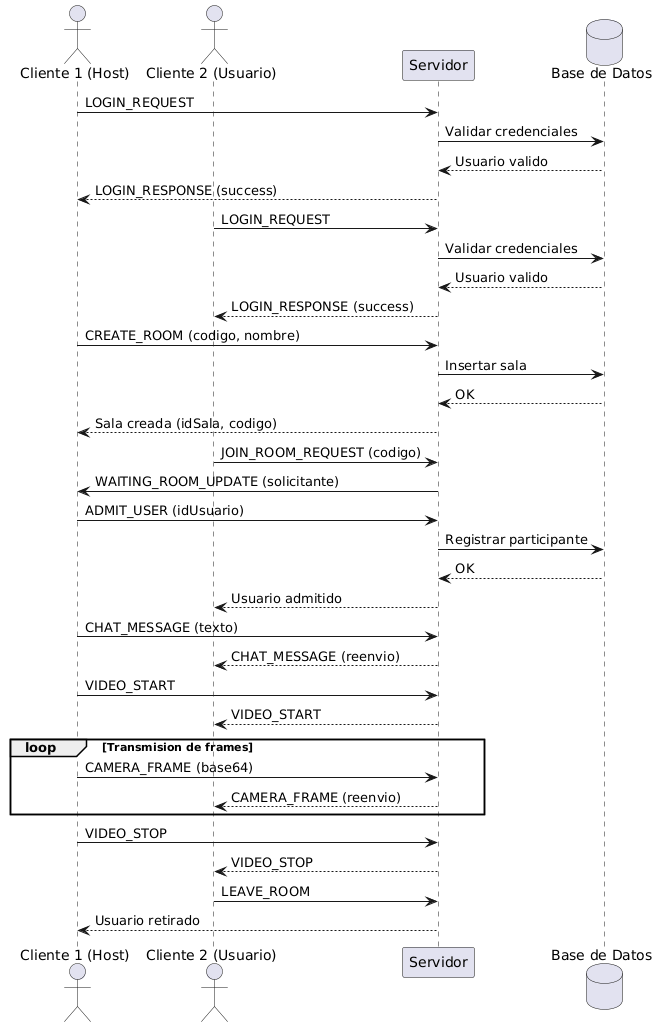
\includegraphics[width=0.9\textwidth]{imagenes/secuencia.png}
    \caption{Diagrama de secuencia del flujo de la aplicaci\'on}
\end{figure}
}{}

\clearpage
\section{Diagrama de Actividades}

\begin{figure}[H]
    \centering
    
\includegraphics[width=0.7\textwidth, height=0.7\textheight, keepaspectratio]{imagenes/actividades.png}
    \caption{Diagrama de actividades del sistema}
\end{figure}

\clearpage
\begin{landscape}
\thispagestyle{empty}
\section{Diagrama de Clases}
\begin{figure}[H]
    \centering
    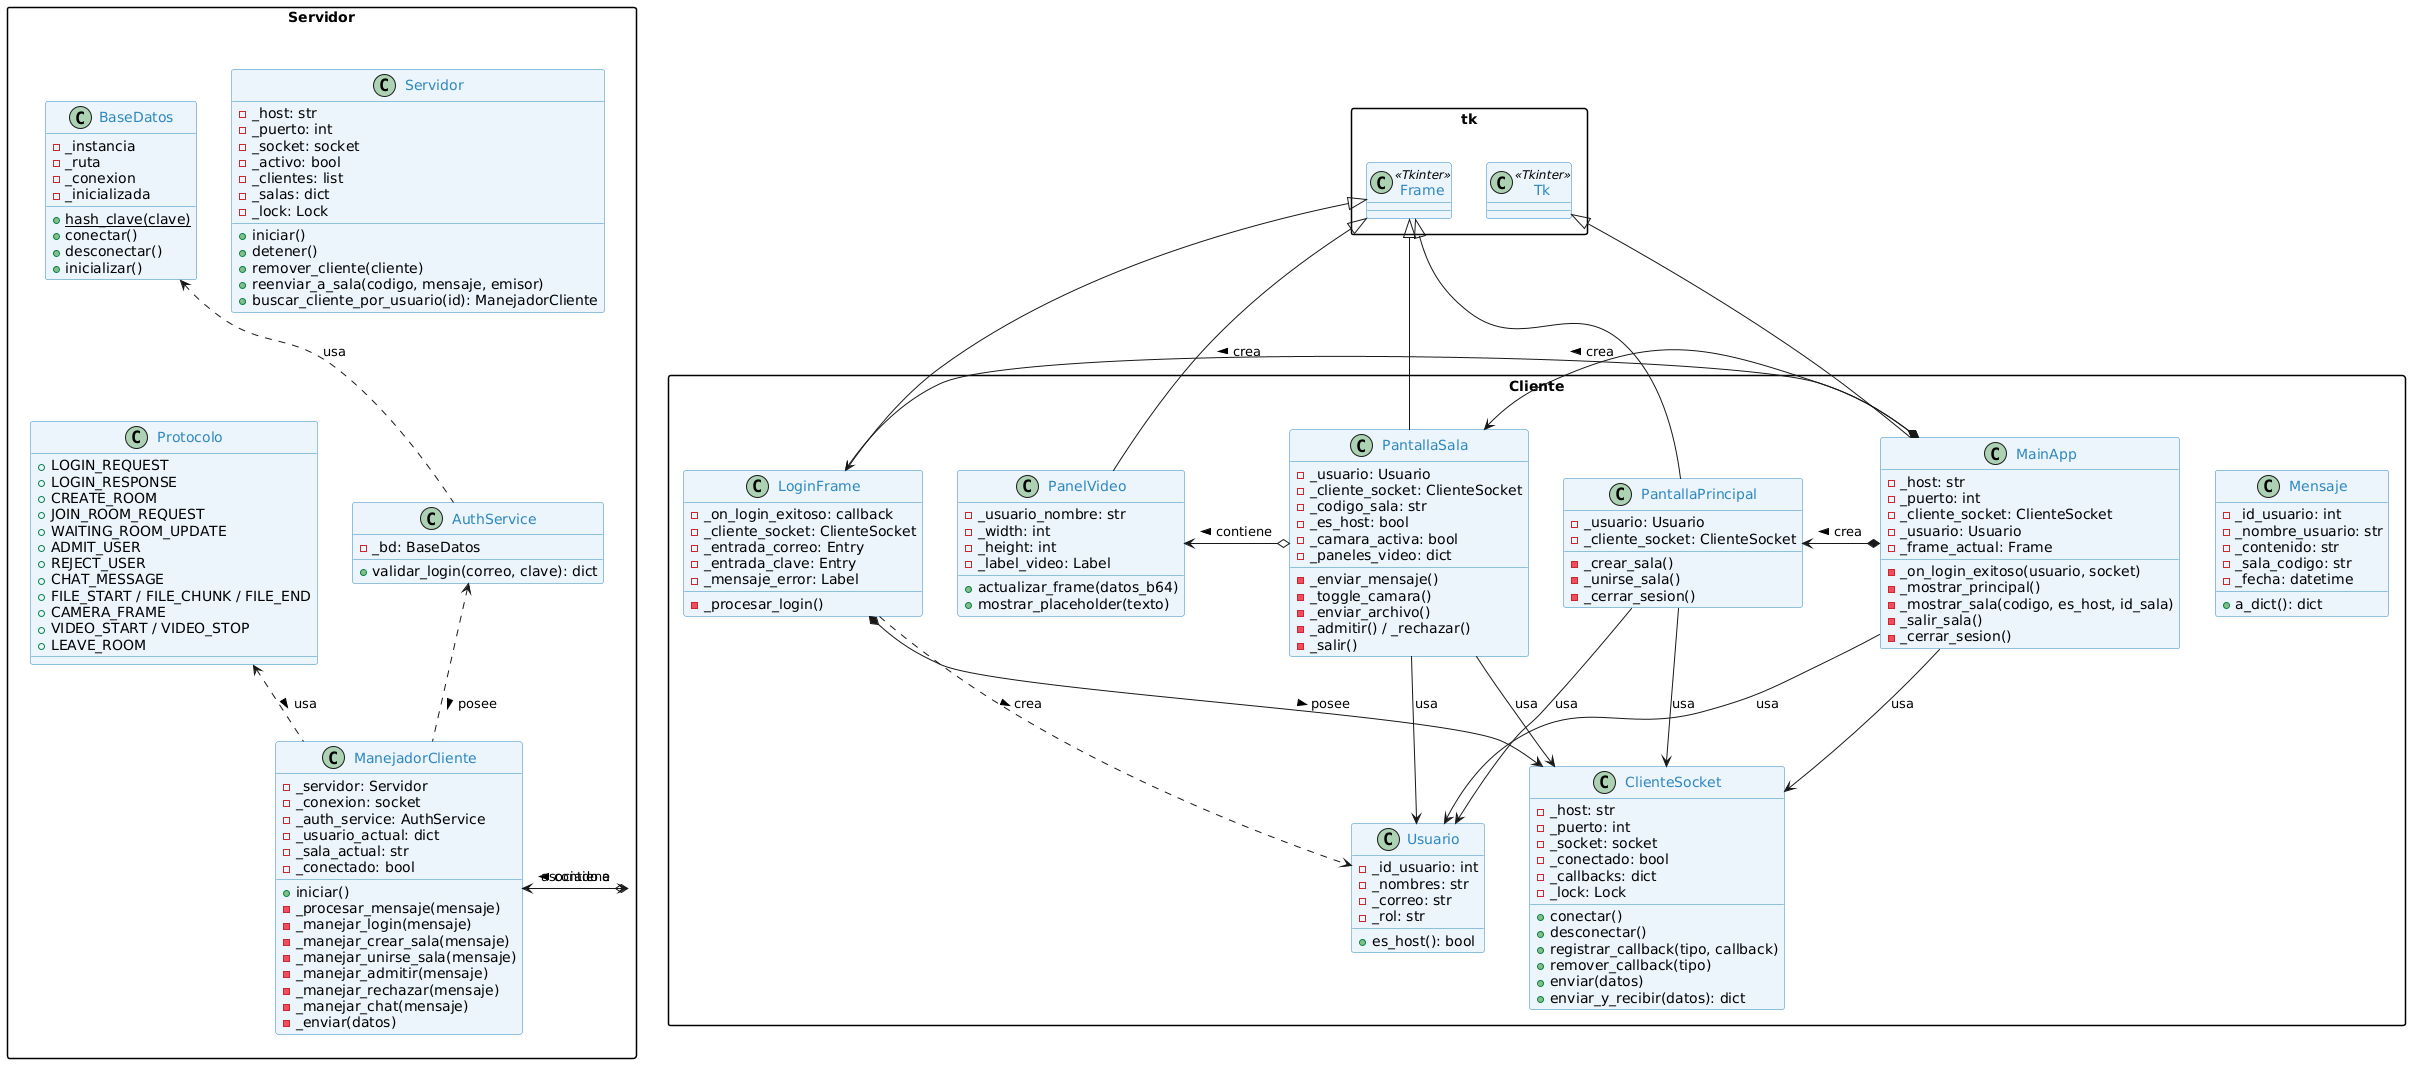
\includegraphics[width=0.95\linewidth, height=0.65\textheight, keepaspectratio]{imagenes/clases.png}
    \caption{Diagrama de clases del sistema}
\end{figure}
\end{landscape}
\clearpage

\section{Descripci\'on del C\'odigo}

Esta secci\'on explica c\'omo funciona cada componente del sistema, detallando el rol de las clases y de qu\'e forma se aplican los principios de la Programaci\'on Orientada a Objetos y los patrones de dise\~no para estructurar una aplicaci\'on modular, escalable y robusta.

\subsection{Funcionamiento de las Clases y Componentes}

El sistema est\'a dividido en tres componentes principales: el Lado del Servidor, el Lado del Cliente y los Gestores de Hardware/Archivos.

\subsubsection{Lado del Servidor}
El servidor gestiona la persistencia de datos y la comunicaci\'on concurrente entre clientes:
\begin{itemize}
    \item \textbf{Protocolo} (\texttt{Servidor/protocolo.py}): Define las constantes de mensaje que viajan serializadas en formato JSON sobre el socket TCP, sirviendo como diccionario del protocolo.
    \item \textbf{BaseDatos} (\texttt{Servidor/base\_datos.py}): Inicializa y mantiene la base de datos SQLite. Centraliza las consultas, registros de salas y autenticaciones.
    \item \textbf{AuthService} (\texttt{Servidor/auth\_service.py}): Valida las credenciales de los usuarios comparando el hash SHA-256 almacenado con el ingresado por el cliente.
    \item \textbf{ManejadorCliente} (\texttt{Servidor/manejador\_cliente.py}): Representa el hilo asignado por el servidor para atender a un cliente. Recibe e interpreta los mensajes JSON delimitados por \verb|\n| y despacha las peticiones.
    \item \textbf{Servidor} (\texttt{Servidor/servidor.py}): Clase principal que abre el socket TCP de escucha, acepta nuevas conexiones de clientes y crea un hilo daemon con su respectivo \texttt{ManejadorCliente}.
\end{itemize}

\subsubsection{Lado del Cliente}
El cliente proporciona la interfaz gr\'afica en Tkinter y procesa la interacci\'on con el usuario y la red:
\begin{itemize}
    \item \textbf{MainApp} (\texttt{Cliente/main.py}): Ventana ra\'iz de Tkinter que administra la transici\'on fluida entre las diferentes vistas de la aplicaci\'on.
    \item \textbf{ClienteSocket} (\texttt{Cliente/cliente\_socket.py}): Abstrae el socket del cliente, manteniendo un hilo de escucha para procesar mensajes entrantes en tiempo real.
    \item \textbf{Modelos} (\texttt{Cliente/modelos/usuario.py, mensaje.py}): Objetos que modelan a un usuario conectado y los mensajes del chat, facilitando su transporte y manipulaci\'on.
    \item \textbf{Pantallas} (\texttt{LoginFrame, PantallaPrincipal, PantallaSala, PanelVideo}): Subclases de Tkinter especializadas en dibujar los formularios de login, el men\'u de salas, la sala de reuniones y las pantallas de video respectivamente.
\end{itemize}

\subsubsection{Gestores de Red y Hardware}
Clases auxiliares delegadas que encapsulan la complejidad de manejar hardware y transmisi\'on:
\begin{itemize}
    \item \textbf{GestorVideo} (\texttt{Cliente/gestores/gestor\_video.py}): Controla la captura de la c\'amara web, decidiendo si usa OpenCV o FFmpeg, y env\'ia los frames comprimidos y codificados en Base64.
    \item \textbf{GestorAudio} (\texttt{Cliente/gestores/gestor\_audio.py}): Captura audio en PCM usando \texttt{sounddevice} y reproduce el audio recibido en un hilo y cola FIFO independientes.
    \item \textbf{GestorArchivos} (\texttt{Cliente/gestores/gestor\_archivos.py}): Controla la transferencia segmentada de archivos en Base64, partiendo el archivo en trozos de 1500 bytes y reconstruy\'endolo en el receptor.
\end{itemize}

\subsection{Aplicaci\'on de los Pilares de la POO}

Los pilares de la Programaci\'on Orientada a Objetos se aplican directamente en la estructuraci\'on de la aplicaci\'on para resolver problemas de modularidad y acoplamiento:

\subsubsection{Encapsulamiento}
Se utiliza para proteger el estado interno de los objetos, ocultando los sockets directos, colecciones de clientes o contrase\~nas, y exponi\'endolas solo mediante m\'etodos o propiedades controladas.
Por ejemplo, en la clase \texttt{Usuario} (\texttt{Cliente/modelos/usuario.py}), los datos del perfil est\'an protegidos con prefijos de guion bajo, y el acceso se restringe mediante decoradores \texttt{@property}. En el servidor, la lista de clientes conectados se protege detr\'as de un lock para evitar condiciones de carrera:

\begin{lstlisting}
class Usuario:
    def __init__(self, id_usuario, nombres, correo, rol):
        self._id_usuario = id_usuario  # Atributo privado
        self._nombres = nombres
        self._rol = rol

    @property
    def id_usuario(self):
        return self._id_usuario

    def es_host(self):
        return self._rol.lower() == "host"
\end{lstlisting}

\subsubsection{Herencia}
Se implementa principalmente en la interfaz gr\'afica para reutilizar los componentes visuales de Tkinter. Clases como \texttt{MainApp} heredan de \texttt{tk.Tk}, y las pantallas (\texttt{LoginFrame}, \texttt{PantallaPrincipal}, \texttt{PantallaSala}, \texttt{PanelVideo}) heredan de \texttt{tk.Frame}, permitiendo extender y personalizar el comportamiento de contenedores gr\'aficos est\'andar:

\begin{lstlisting}
class PanelVideo(tk.Frame):  # Hereda de tk.Frame
    def __init__(self, master, usuario_nombre="", width=240, height=180, bg="#222"):
        super().__init__(master, bg=bg, width=width, height=height)
        self.pack_propagate(False)
        # Widgets especificos para dibujar el video
\end{lstlisting}

\subsubsection{Polimorfismo}
Permite tratar de forma homog\'enea diferentes pantallas dentro del flujo de la aplicaci\'on. En \texttt{MainApp}, la variable \texttt{\_frame\_actual} puede contener instancias de \texttt{LoginFrame}, \texttt{PantallaPrincipal} o \texttt{PantallaSala}. Al cambiar de pantalla, el contenedor llama polim\'orficamente a los m\'etodos heredados como \texttt{pack()} y \texttt{destroy()}:

\begin{lstlisting}
# Transicion dinamica de pantallas en MainApp
self._frame_actual.destroy()  # Destruye la pantalla previa
self._frame_actual = PantallaSala(self, ...)  # Instancia nueva pantalla
self._frame_actual.pack(fill=tk.BOTH, expand=True)  # Empaqueta polimorficamente
\end{lstlisting}

\subsubsection{Abstracci\'on}
Oculta la complejidad t\'ecnica de la red y el hardware de las pantallas de usuario. \texttt{ClienteSocket} encapsula toda la l\'ogica del socket TCP, serializaci\'on JSON y buffer, ofreciendo solo m\'etodos de alto nivel como \texttt{enviar} o \texttt{registrar\_callback}:

\begin{lstlisting}
class ClienteSocket:
    def conectar(self): ...
    def enviar(self, datos):
        self._socket.send((json.dumps(datos) + "\n").encode("utf-8"))
    def registrar_callback(self, tipo, callback):
        self._callbacks[tipo] = callback
\end{lstlisting}

\subsection{Patrones de Dise\~no Implementados}

Los patrones de dise\~no se utilizaron para dar una soluci\'on limpia y estandarizada a las problem\'aticas t\'ipicas de una aplicaci\'on cliente-servidor:

\subsubsection{Singleton (Instancia \'{U}nica)}
Garantiza que la clase \texttt{BaseDatos} posea una \'unica instancia en todo el ciclo del servidor, centralizando las conexiones y evitando fallos por concurrencia en SQLite:

\begin{lstlisting}
class BaseDatos:
    _instancia = None

    def __new__(cls, *args, **kwargs):
        if cls._instancia is None:
            cls._instancia = super().__new__(cls)
        return cls._instancia
\end{lstlisting}

\subsubsection{Observer (Observador)}
El \texttt{ClienteSocket} act\'ua como sujeto que recibe mensajes de la red, y las diferentes pantallas o gestores se registran como observadores a trav\'es de callbacks, recibiendo notificaciones cuando se detecta un mensaje que les compete:

\begin{lstlisting}
# Suscripcion (Observadores se registran)
self._cliente_socket.registrar_callback("CHAT_MESSAGE", self._recibir_chat)

# Notificacion en ClienteSocket
def _escuchar(self):
    ...
    cb = self._callbacks.get(mensaje.get("type"))
    if cb:
        cb(mensaje)  # Notifica al callback registrado
\end{lstlisting}

\subsubsection{Strategy (Estrategia)}
El \texttt{GestorVideo} define algoritmos de captura de video intercambiables. Si el cliente dispone de OpenCV instalado en su sistema, el gestor utiliza \texttt{cv2.VideoCapture} para capturar los frames; en caso contrario, alterna a una estrategia basada en \texttt{ffmpeg} leyendo directamente desde el dispositivo de video local:

\begin{lstlisting}
def _capturar_y_enviar(self):
    if self._backend == "opencv":
        self._capturar_con_opencv()
    else:
        self._capturar_con_ffmpeg()
\end{lstlisting}

\subsubsection{Facade (Fachada)}
El \texttt{ManejadorCliente} en el servidor funciona como una fachada que centraliza y simplifica el uso de m\'ultiples subsistemas complejos del servidor (como \texttt{AuthService}, \texttt{BaseDatos} y la distribuci\'on de mensajes de \texttt{Servidor}), exponiendo solo una interfaz simple mediante el m\'etodo \texttt{iniciar()}.

\subsubsection{Command (Comando)}
El protocolo de red encapsula las intenciones del usuario en objetos JSON que viajan por el socket con un campo \texttt{type} que act\'ua como comando. Esto permite enrutar y procesar de forma gen\'erica las peticiones:

\begin{lstlisting}
# Servidor interpreta y despacha comandos de forma desacoplada
if tipo == Protocolo.LOGIN_REQUEST:
    self._manejar_login(mensaje)
elif tipo == Protocolo.CREATE_ROOM:
    self._manejar_crear_sala(mensaje)
\end{lstlisting}

\subsubsection{Factory Method (M\'etodo F\'abrica)}
\texttt{MainApp} delega la creaci\'on e instanciaci\'on de las pantallas visuales a m\'etodos f\'abrica espec\'ificos (\texttt{\_mostrar\_login()}, \texttt{\_mostrar\_principal()}, \texttt{\_mostrar\_sala()}). El cliente no conoce c\'omo se construyen las pantallas, solo invoca la f\'abrica:

\begin{lstlisting}
def _mostrar_sala(self, codigo_sala, es_host, id_sala):
    self._frame_actual = PantallaSala(self, self._usuario, self._cliente_socket, codigo_sala, es_host, id_sala, self._salir_sala)
    self._frame_actual.pack(fill=tk.BOTH, expand=True)
\end{lstlisting}

\subsubsection{Template Method (M\'etodo Plantilla)}
En la transmisi\'on de video, la captura e inicializaci\'on siguen un esqueleto predefinido (establecer conexi\'on, inicializar buffer, iterar captura, codificar, enviar y liberar recursos). La l\'ogica del bucle de captura se define en la superclase del gestor, mientras que los pasos espec\'ificos para la lectura de la c\'amara cambian seg\'un la estrategia.

\section{Protocolos y Normativas Utilizados}

El sistema utiliza \textbf{TCP} como protocolo de transporte para todas las comunicaciones. Cada funcionalidad prepara el dato de forma distinta antes de enviarlo, pero todas comparten el mismo canal confiable.

\begin{itemize}
    \item \textbf{Video:} la c\'amara es capturada por OpenCV (o ffmpeg). El frame se comprime en formato JPEG y se convierte a texto mediante Base64 para poder viajar dentro de un mensaje JSON. Elegimos TCP para transportar esos frames entre m\'aquinas --- aunque en sistemas reales como Zoom se usa UDP para menor latencia.
    \item \textbf{Audio:} el micr\'ofono entrega bloques de audio crudo (PCM). Esos bytes tambi\'en se convierten a Base64 y se env\'ian por TCP. El receptor los reproduce en orden mediante una cola interna.
    \item \textbf{Archivos:} el archivo se lee completo, se codifica en Base64 y se corta en pedazos peque\~nos. Se env\'ian con un mensaje de inicio, varios fragmentos y uno de fin --- as\'{\i} el receptor sabe cu\'ando rearmar el archivo original.
    \item \textbf{Mensajes de control} (login, crear sala, chat, etc.): viajan directamente como objetos JSON sobre TCP, delimitados por el car\'acter \verb|\n|.
\end{itemize}

\subsection{Tabla de Mensajes del Protocolo}

Los mensajes se env\'ian en JSON sobre TCP, delimitados por \verb|\n|.

\begin{table}[htbp]
    \centering
    \small
    \begin{tabular}{>{\raggedright\arraybackslash}p{4.5cm}p{2.5cm}p{8.5cm}}
    \toprule
    \textbf{Tipo} & \textbf{Direcci\'on} & \textbf{Campos} \\
    \midrule
    LOGIN\_REQUEST   & Cliente $\rightarrow$ Servidor & correo, clave \\
    LOGIN\_RESPONSE  & Servidor $\rightarrow$ Cliente & status, idUsuario, nombres, rol \\
    CREATE\_ROOM     & Cliente $\rightarrow$ Servidor & codigo, nombre, idHost \\
    JOIN\_ROOM\_REQUEST & Cliente $\rightarrow$ Servidor & codigo, idUsuario \\
    WAITING\_ROOM\_UPDATE & Servidor $\rightarrow$ Host & idSala, solicitanteId, solicitanteNombre \\
    ADMIT\_USER      & Host $\rightarrow$ Servidor & idSala, idUsuario \\
    REJECT\_USER     & Host $\rightarrow$ Servidor & idSala, idUsuario \\
    CHAT\_MESSAGE    & Cliente $\rightarrow$ Sala & roomCode, userName, message \\
    FILE\_START      & Cliente $\rightarrow$ Sala & roomCode, fileName, fileSize \\
    FILE\_CHUNK      & Cliente $\rightarrow$ Sala & roomCode, fileName, data \\
    FILE\_END        & Cliente $\rightarrow$ Sala & roomCode, fileName \\
    CAMERA\_FRAME    & Cliente $\rightarrow$ Sala & roomCode, userName, data (base64) \\
    VIDEO\_START     & Cliente $\rightarrow$ Sala & roomCode, userName \\
    VIDEO\_STOP      & Cliente $\rightarrow$ Sala & roomCode, userName \\
    LEAVE\_ROOM      & Cliente $\rightarrow$ Servidor & roomCode \\
    \bottomrule
    \end{tabular}
    \caption{Tipos de mensaje del protocolo}
\end{table}

\section{Manual de Instalaci\'on y Ejecuci\'on}

\subsection{Requisitos}
\begin{itemize}
    \item Python 3.10 o superior
    \item Pillow (instalar con \texttt{pip install -r requirements.txt})
    \item Opcional: OpenCV (\texttt{pip install opencv-python}) o ffmpeg
\end{itemize}

\subsection{Ejecuci\'on}
\begin{enumerate}
    \item Iniciar el servidor:
    \begin{lstlisting}
python -m Servidor.servidor
    \end{lstlisting}
    \item Iniciar uno o m\'as clientes:
    \begin{lstlisting}
python -m Cliente.main
    \end{lstlisting}
\end{enumerate}

\subsection{Datos de Prueba}

\begin{table}[htbp]
    \centering
    \begin{tabular}{p{2.5cm}p{3cm}p{1.5cm}p{1.5cm}}
    \toprule
    \textbf{Nombre} & \textbf{Correo} & \textbf{Clave} & \textbf{Rol} \\
    \midrule
    Luis Tasayco  & luis@email.com   & 123456 & Host \\
    Ana Torres    & ana@email.com    & 123456 & Usuario \\
    Carlos Ruiz   & carlos@email.com & 123456 & Usuario \\
    \bottomrule
    \end{tabular}
    \caption{Usuarios de prueba}
\end{table}

\section{Conclusiones}

\begin{itemize}
    \item Se implement\'o un prototipo funcional de videoconferencia con arquitectura cliente-servidor.
    \item Los sockets TCP con protocolo JSON proporcionan una base s\'olida para comunicaci\'on en tiempo real.
    \item Los cuatro pilares de la POO -- encapsulamiento, herencia, polimorfismo y abstracci\'on -- fueron aplicados consistentemente en todo el c\'odigo.
    \item Se identificaron y aplicaron siete patrones de dise\~no: Singleton, Observer, Strategy, Facade, Command, Template Method y Factory Method.
    \item La POO permiti\'o organizar el c\'odigo en clases especializadas con responsabilidades claras.
    \item La concurrencia con hilos permite atender m\'ultiples clientes simult\'aneamente.
    \item La transmisi\'on de video se logr\'o mediante captura, compresi\'on JPEG y codificaci\'on base64.
\end{itemize}

\end{document}
